%%%%%%%%%%%%%%%%%%%%%%%%%%%%%%%%%%%%%%%%%%
% Engineering problems / LaTeX Template
%		Semester 6
%		Institut d'Optique Graduate School
%%%%%%%%%%%%%%%%%%%%%%%%%%%%%%%%%%%%%%%%%%
%	6N-IntNum-BlocCamera	/ Industrial Sensor
%%%%%%%%%%%%%%%%%%%%%%%%%%%%%%%%%%%%%%%%%%
%
% Created by:
%	Julien VILLEMEJANE - 16/jul/2024
% Fichier.sty modifié pour changer la police de caractère
%	
%
%%%%%%%%%%%%%%%%%%%%%%%%%%%%%%%%%%%%%%%%%%
% Professional Newsletter Template
% LaTeX Template
% Version 1.0 (09/03/14)
%
% Created by:
% Bob Kerstetter (https://www.tug.org/texshowcase/) and extensively modified by:
% Vel (vel@latextemplates.com)
% 
% This template has been downloaded from:
% http://www.LaTeXTemplates.com
%
% License:
% CC BY-NC-SA 3.0 (http://creativecommons.org/licenses/by-nc-sa/3.0/)
%
%%%%%%%%%%%%%%%%%%%%%%%%%%%%%%%%%%%%%%%%%

\documentclass[a4paper,11pt,titlepage]{article} % The default font size is 10pt; 11pt and 12pt are alternatives

%%%%%%%%%%%%%%%%%%%%%%%%%%%%%%%%%%%%%%%%%%%%%%%%%%%%%%%%%%%%%%%%%%%%%%%%%%%%%%%%%%%%%%%%%%%%%%%%%%%%%%%%%%%%%%%%%%%%%%%%%%%%%%%%%%%%%%%%%%%%%%%%%%%%%%%%%%%%%%%%%%%%%%%%%%%%%%%%%%%%%%%%%%%%%%%%%%%%%%%%%%%%%%%%%%%%%%%%%%%%%%%%%%%%%%%%%%%%%%%%%%%%%%%%%%%%
\usepackage{opto_elec_villemejane}

%%%%%%%%%%%%%%%%%%%%%%%%%%%%%%%%%%%%%%%%%%%%%%%%
%%%%%%%%%%%%%%%%%%%%%%%%%%%%%%%%%%%%%%%%%%%%%%%%
\begin{document}



% Page de garde
\begin{titlepage}

\begin{center}
	\begin{minipage}{2.5cm}
	\begin{center}
		
\includegraphics[width=8cm]{images/Logo-LEnsE.png}
	\end{center}
\end{minipage}\hfill
\begin{minipage}{10cm}
	\begin{center}
	\textbf{Institut d'Optique Graduate School }\\[0.1cm]
    \textbf{Interfaçage Numérique}


	\end{center}
\end{minipage}\hfill


\vspace{4cm}


{\huge \bfseries \textsc{Interfaçage Numérique}} \\[0.5cm]
{\large \bfseries Travaux Pratiques} \\[0.2cm]
Semestre 6

\vspace{1.2cm}
% Title
\rule{\linewidth}{0.3mm} \\[0.4cm]
{ \huge \bfseries\color{violet_iogs} Chaine d'acquisition d'une image \\ Manipulation d'images\\[0.4cm] }
\rule{\linewidth}{0.3mm} \\[0.8cm]

2 séances

\bigskip

\begin{center}
	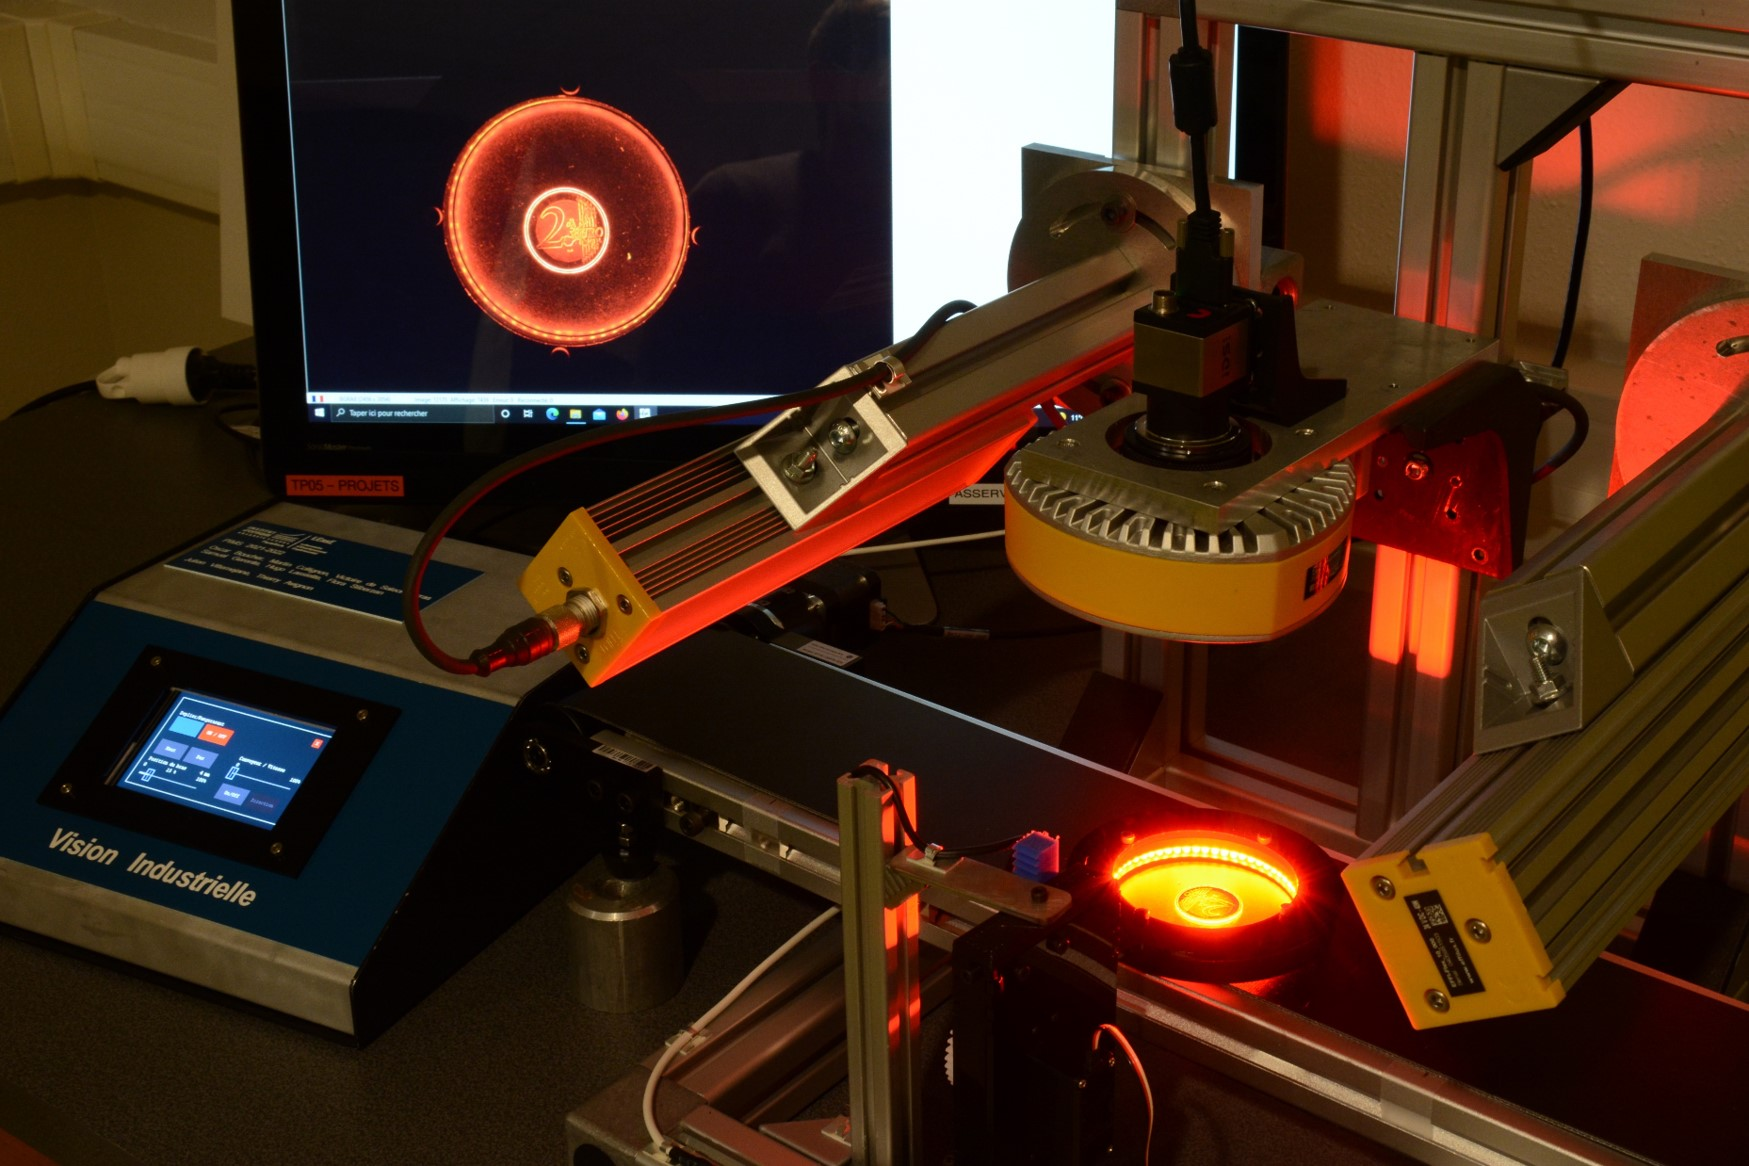
\includegraphics[width=0.5\textwidth]{images/camera_vi.jpg}
\end{center}

\bigskip

\vfill

\textit{Ce sujet est disponible au format électronique sur le site du LEnsE - https://lense.institutoptique.fr/ dans la rubrique Année / Première Année / Interfaçage Numérique S6 / Bloc Caméra.}

% Bottom of the page
%{\textbf{\large {Année universitaire} 2024-2025}}

\end{center}
\end{titlepage}

\newpage
\strut % empty page


%%%%%%%%%%%%%%%%%%%%%%%%%%%%%%%%%%%%%%%%%%%%%%%%
%%%%%%%%%%%%%    Intro
\newpage
\pagestyle{empty}

\begin{minipage}[c]{.25\linewidth}
	
\includegraphics[width=5cm]{images/Logo-LEnsE.png}
\end{minipage} \hfill
\begin{minipage}[c]{.4\linewidth}

\begin{center}
\vspace{0.3cm}
{\Large \textsc{Interfaçage Numérique}}

\medskip

6N-047-SCI \qquad \textbf{\Large Bloc Caméra}

\end{center}
\end{minipage}\hfill

\vspace{0.5cm}

\noindent \rule{\linewidth}{1pt}

{\noindent\Large  \rule[-7pt]{0pt}{30pt} \textbf{Chaine d'acquisition d'une image et manipulation d'images avec OpenCV}}

\noindent \rule{\linewidth}{1pt}

\bigskip

%%%%%%%%%%%%%%%%%%%%%%%%%%%%%%%%%%%%%%%%%%%%%%%%
%%%%%%%%%%%%%    Objectifs

\section{Objectifs du bloc}

L'objectif principal de ce bloc est de découvrir les \textbf{différents paramètres impactant la qualité d'une prise d'image par une caméra} dans un environnement industriel ainsi que la \textbf{manipulation d'images numériques}, à l'aide de la bibliothèque \textbf{OpenCV}.

On s'intéressera à l'impact du \textbf{temps d'intégration}, de la \textbf{résolution} de la caméra et de l'\textbf{éclairage} (couleur et intensité) de la scène et des objets sur l'image résultante. 


\noindent \rule{\linewidth}{1pt}

\medskip

%%%%%%%%%%%%%%%%%%%%%%%%%%%%%%%%%%%%%%%%%%%%%%%%
%%%%%%%%%%%%%    A A V

À l'issue des séances de TP concernant le bloc sur les caméras industrielles et la manipulation d'images, les étudiant$\cdot$es seront capables de~:

\begin{itemize}
	\item paramétrer le temps d'exposition en fonction de l'intensité lumineuse pour \textbf{obtenir une image d'une qualité exploitable}
	\item utiliser des outils d'analyse (histogramme notamment) pour \textbf{améliorer numériquement} la qualité d'une image (contraste, luminosité...)
	\item \textbf{manipuler une image numérique} à l'aide de la bibliothèque \textsl{OpenCV}
	% \item \textbf{extraire des primitives} de bas niveau dans une image.
\end{itemize}

\noindent \rule{\linewidth}{1pt}


\textit{Cette étude sera complétée par un TP plus détaillé sur les bruits associés à l'utilisation des caméras CMOS en 2ème année du cycle ingénieur à Palaiseau.}

\textit{Des cours et des projets autour du traitement d'images sont également proposés dans les prochaines années de formation, quelque soit le site. Ces deux séances sont une introduction à ces modules plus avancés.}

\textit{Le bloc \textbf{Images et OpenCV} (facultatif) de ce module permet d'aller également plus loin dans le pré-traitement des images et leur manipulation.}


%%%%%%%%%%%%%%%%%%%%%%%%%%%%%%%%%%%%%%%%%%%%%%%%
%%%%%%%%%%%%%    Ressources

\section{Ressources}
\begin{itemize}
	\item ??
\end{itemize}


\newpage
%%%%%%%%%%%%%%%%%%%%%%%%%%%%%%%%%%%%%%%%%%%%%%%%
%%%%%%%%%%%%%    Déroulement
\section{Déroulement du bloc}

\subsection{Séance 1 - Modélisation primaire d'une chaine d'acquisition}
\begin{description}
	\item[Etape 0 - 30 min] Prendre en main l'interface de pilotage
	\item[Etape 1 - 30 min] Décrire le rôle des principales caractéristiques d'une caméra CMOS (temps d'intégration, black level...) 
	\item[Etape 2 - 30 min] Analyser la pertinence de l'éclairage sur une scène à l'aide de l'histogramme d'une image
	\item[Etape 3 - 30 min] Analyser l'impact du choix de la couleur de l'éclairage en fonction des caractéristiques d'un objet
	\item[Etape 4 - 30 min] Analyser l'impact de l'échantillonnage et la quantification sur les images
	\item[Etape 5 - 30 min] \textit{Réponse de la caméra}
	\item[Etape 6 - 60 min] Analyser l'impact des outils de base de la manipulation d'images (\textit{Contraste, luminosité, seuillage et filtrage})
\end{description}
	
\subsection{Séance 2 - Manipulation d'images}
\begin{description}
	\item[Etape 1 - 20 min] Ouvrir une image sous OpenCV (niveau de gris et couleur) et extraire les informations utiles de l'image
	\item[Etape 2 - 20 min] Calculer l'histogramme d'une image et l'afficher
	\item[Etape 3 - 20 min] Améliorer numériquement la qualité d'une image : contraste, luminosité...
	\item[Etape 4 - 90 min] Appliquer un filtre moyenneur (\textit{Gaussian blur}) sur une image et analyser l'impact du choix du noyau
	\item[Etape 5 - 60 min] Appliquer un filtre passe-haut (\textit{Roberts, Sobel}) sur une image et analyser l'impact du choix du noyau
	\item[Etape 6 - 30 min] Appliquer un filtre par l'intermédiaire de la transformée de Fourier
\end{description}

\noindent \rule{\linewidth}{1pt}

\medskip



\newpage
\strut % empty page
%%%%%%%%%%%%%%%%%%%%%%%%%%%%%%%%%%%%%%%%%%%%%%%%
%%%%%%%%%%%%%    Séance 1 détaillée

\begin{minipage}[c]{.25\linewidth}
	
\includegraphics[width=4cm]{images/Logo-LEnsE.png}
\end{minipage} \hfill
\begin{minipage}[c]{.4\linewidth}

\begin{center}
\vspace{0.3cm}
{\Large \textsc{Interfaçage Numérique}}

\medskip

6N-047-SCI \qquad \textbf{\Large Bloc Caméra}

\end{center}
\end{minipage}\hfill

\vspace{0.5cm}

\noindent \rule{\linewidth}{1pt}

{\noindent\Large \rule[-7pt]{0pt}{30pt} \textbf{Séance 1} / Modélisation primaire d'une chaine d'acquisition} 

\noindent \rule{\linewidth}{1pt}

Ce bloc de travaux pratiques utilise un \textbf{banc de vision industrielle} avec une lampe de type Effi-Ring RGB, une caméra Basler et une interface développée en \textbf{Python} (\textit{PyQt6}) et qui utilise des fonctionnalités de la bibliothèque \textbf{OpenCV}.

Les documentations de la caméra et de l'éclairage sont disponibles aux adresses suivantes : 

\begin{itemize}
	\item Basler \textbf{a2A 1920 - 160ucBAS} : \href{https://docs.baslerweb.com/a2a1920-160ucbas#specifications}{https://docs.baslerweb.com/a2a1920-160ucbas\#specifications}
	\item \textbf{Effi-Ring} : \href{https://www.effilux.com/fr/produits/annulaire/effi-ring}{https://www.effilux.com/fr/produits/annulaire/effi-ring}
\end{itemize}

%%%%%%%%%%%%%%%%%%%%%%%%%%%%%%%%%%%%%%%%%%%%%%%%
%%%%%%%%%%%%%    Déroulement détaillé

%%%%%%%%%%%%%    Etape 0
\section{Prise en main de l'interface}

\begin{center} \textbf{\textit{Temps conseillé : 30 min}} \end{center}

\Manip Lancer l'application CMOS\_Machine\_Vision depuis ...

(pour l'instant dernière version officielle sur le github suivant : 

https://github.com/IOGS-LEnsE-ressources/camera-gui  

-  répertoire applis/CMOS-MachineVision\_v3  )

\begin{center}
	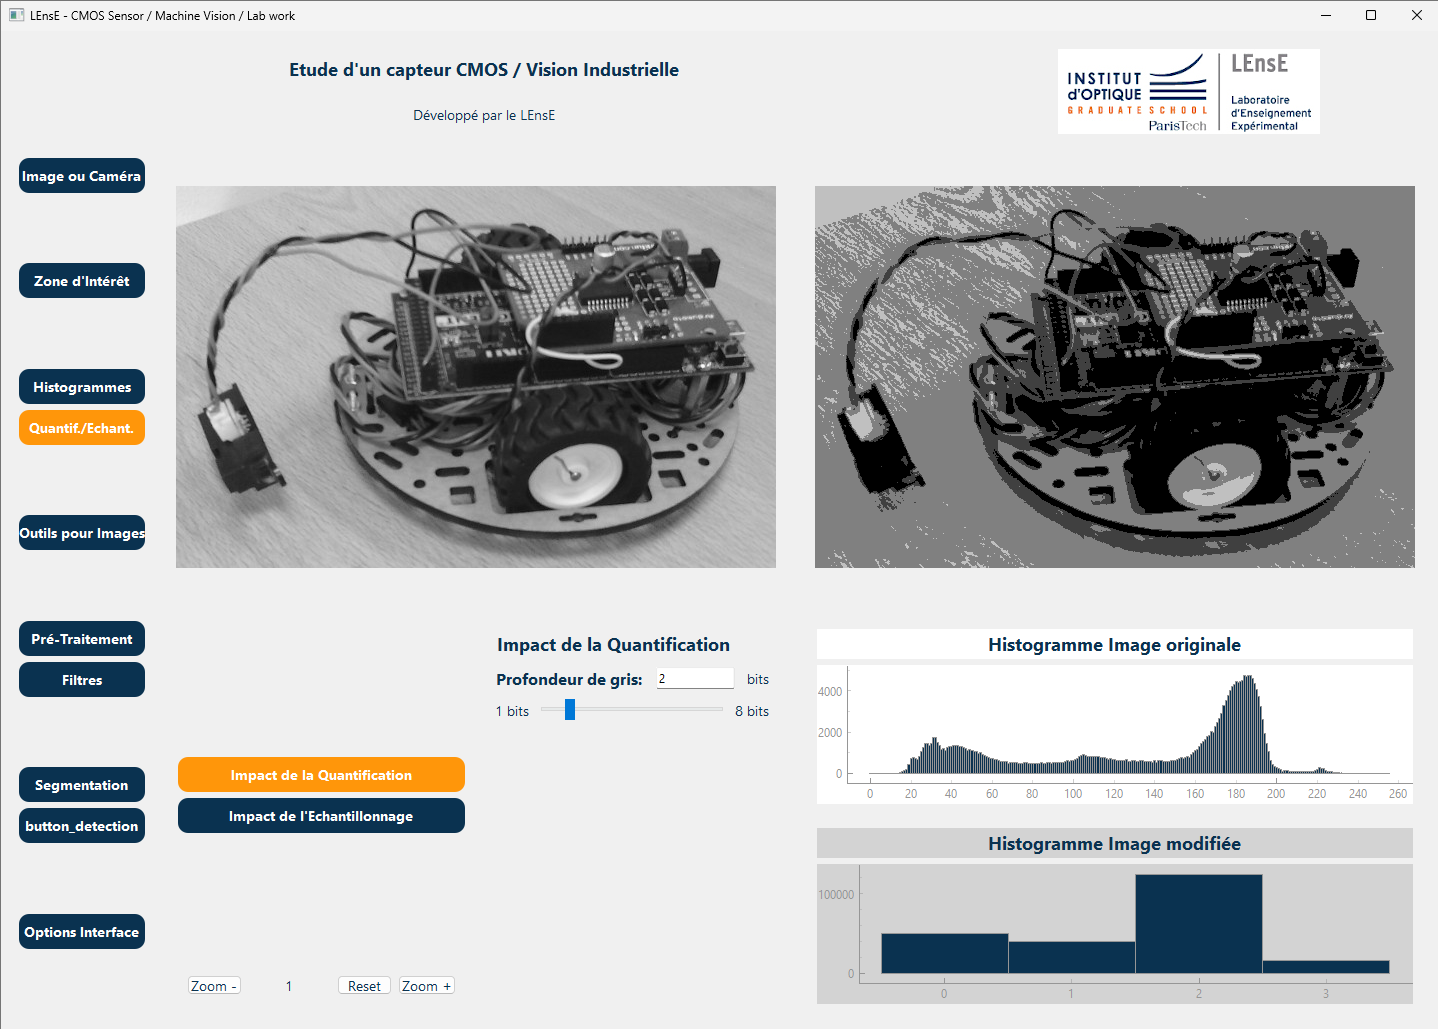
\includegraphics[width=0.9\textwidth]{./images/camera_gui.png}
\end{center}


\Manip Ouvrir la première caméra disponible dans l'onglet \textsc{Image ou Caméra} / \textsc{Sélectionner une caméra} / \textsc{Ouvrir la première caméra}.

\subsection{Eclairage et zone d'intérêt}

\Manip Allumer l'éclairage annulaire du banc (trois couleurs). 

\Quest Quelle couleur d'éclairage obtient-on ?

\Manip Placer un objet (un cube de couleur par exemple) dans le champ de la caméra.

\Manip Ajuster la zone d'intérêt (ou \textit{Area of Interest} - AOI) à l'aide de l'onglet \textsc{Zone d'Intérêt} pour ne sélectionner qu'une partie de l'image autour de l'objet.

\Quest Que pouvez-vous dire des deux histogrammes affichés ?


%%%%%%%%%%%%%    Etape 1

\section{Décrire le rôle des principales caractéristiques d'une caméra CMOS}

\begin{center} \textbf{\textit{Temps conseillé : 30 min}} \end{center}


\subsection{Temps d'intégration}

\Manip Dans l'onglet \textsc{Image ou Caméra}, sélectionner un \textit{Black Level} de 0. Modifier le temps d'intégration de la caméra.

\Quest Que constatez-vous sur l'histogramme de l'image ? Sur la moyenne et l'écart-type de la répartition de la luminosité des pixels ?

\Manip Placer un cache devant la caméra (ou Prévoir une caméra annexe avec cache - pour éviter d'enlever l'objectif et mettre un cache...) pour vous placer dans l'obscurité.

\Quest La répartition de la luminosité perçu par chaque pixel est-elle uniforme ? Que pouvez-vous en conclure ?

\subsection{Black Level}

\Manip Dans l'obscurité, relever l'histogramme de l'image ainsi que la moyenne et l'écart-type de la répartition de la luminosité des pixels pour différentes valeurs du \textit{black level} : 0, 10, 20, 50.

\Quest Que peut-on conclure de l'intérêt du black level ?


%%%%%%%%%%%%%    Etape 2
\section{Analyser la pertinence de l'éclairage d'une scène}

\begin{center} \textbf{\textit{Temps conseillé : 30 min}} \end{center}

Utilisation de l'histogramme et du seuillage par exemple pour définir le bon éclairage permettant de séparer l'objet du fond ?

Trouver des échantillons pertinents.


%%%%%%%%%%%%%    Etape 3
\section{Analyser l'impact du choix de la couleur de l'éclairage}

\begin{center} \textbf{\textit{Temps conseillé : 30 min}} \end{center}


Caméra monochrome : quelle couleur d'éclairage pour détecter la couleur d'un objet ? (premier pas vers colorimétrie/photométrie)

Trouver des objets qui ont des comportements similaires en GRAY avec des couleurs différentes.


%%%%%%%%%%%%%    Etape 4
\section{Analyser l'impact de l'échantillonnage et la quantification sur les images}

\begin{center} \textbf{\textit{Temps conseillé : 30 min}} \end{center}


\subsection{Matériel}

Objets de tailles différentes, de formes différentes...

Mire papier dans le champ de la caméra pour faire des mesures ?

Trouver un échantillon (ou une image préenregistrée) permettant par sous-échantillonnage d'obtenir un autre motif (Moiré)

\subsection{Questions }

--> Quelle est l'influence du choix d'un pas de quantification ?

--> Quelle est l'influence du choix d'un pas d'échantillonnage ?


%%%%%%%%%%%%%    Etape 5
\section{Réponse de la caméra}

\begin{center} \textbf{\textit{Temps conseillé : 30 min}} \end{center}

A partir des spectres des sources RGB, essayer (sur un même objet - ayant des propriétés quasi équivalentes en reflexion quelque soit la longueur d'onde du visible) de caractériser la courbe de réponse de la caméra ? 

Avec une lumière blanche et des filtres ?


%%%%%%%%%%%%%    Etape 6
\section{Analyser l'impact des outils de base de la manipulation d'images}

\begin{center} \textbf{\textit{Temps conseillé : 60 min}} \end{center}

Via l'interface, jouer sur \textit{Contraste, luminosité, seuillage et filtrage} et voir l'effet sur l'histogramme et sur l'image.

\newpage
\strut % empty page
%%%%%%%%%%%%%%%%%%%%%%%%%%%%%%%%%%%%%%%%%%%%%%%%
%%%%%%%%%%%%%    Séance 2 détaillée
\begin{minipage}[c]{.25\linewidth}
	
\includegraphics[width=4cm]{images/Logo-LEnsE.png}
\end{minipage} \hfill
\begin{minipage}[c]{.4\linewidth}

\begin{center}
\vspace{0.3cm}
{\Large \textsc{Interfaçage Numérique}}

\medskip

6N-047-SCI \qquad \textbf{\Large Bloc Caméra}

\end{center}
\end{minipage}\hfill

\vspace{0.5cm}

\noindent \rule{\linewidth}{1pt}

{\noindent\Large \rule[-7pt]{0pt}{30pt} \textbf{Séance 2} / Manipulation d'images (OpenCV) et filtrage} 

\noindent \rule{\linewidth}{1pt}

Lors de cette séance, vous devrez écrire vos propres scripts en \textbf{Python} (avec l'IDE PyCharm par exemple) permettant de réaliser des opérations de base de manipulation d'images, à l'aide notamment de la célèbre bibliothèque \textbf{OpenCV}.

\section{Ressources}

Un tutoriel sur les bases d'OpenCV est disponible à l’adresse suivante : 

\href{https://iogs-lense-training.github.io/image-processing/}{https://iogs-lense-training.github.io/image-processing/}

Un \textbf{kit d'images} est disponible sur le site du LEnsE dans la rubrique \textit{Année / Première Année / Interfaçage Numérique S6 / Bloc Images et OpenCV / Kit d'images}. 


Diapos : SC19 - Image Processing


%%%%%%%%%%%%%    Etape 1
\section{Ouvrir une image sous OpenCV}

\begin{center} \textbf{\textit{Temps conseillé : 20 min}} \end{center}

\begin{mdframed}[style=sidebar,frametitle={}]
Notions : \href{https://iogs-lense-training.github.io/image-processing/contents/opencv.html#open-an-image
}{\textit{Open an image}} - \href{https://iogs-lense-training.github.io/image-processing/contents/opencv.html#display-an-image
}{\textit{Display an image}}
\end{mdframed}

\Manip Créer un nouveau projet sous PyCharm.

\Manip Impoter la bibliothèque \textbf{OpenCV2} (\textit{cv2}).

\medskip

\textit{Pour la suite, il est nécessaire de placer \textbf{tous les fichiers dans le même dossier} : votre script Python, les
différentes images et les bibliothèques de fonction (fichier \textsl{images\_manipulation.py})}

\Manip Ouvrir l'image \textsl{robot.jpg} du kit d'images fourni, au format RGB.

\Quest Quelle est la taille de l'image ? Quel est le type de données d'un élément ?

\Manip Ouvrir l'image \textsl{robot.jpg} du kit d'images fourni, en niveau de gris.

\Quest Quelle est la taille de l'image ? Quel est le type de données d'un élément ?


%%%%%%%%%%%%%    Etape 2
\section{Calculer l'histogramme d'une image et l'afficher}

\begin{center} \textbf{\textit{Temps conseillé : 20 min}} \end{center}

\begin{mdframed}[style=sidebar,frametitle={}]
Notions : \href{https://iogs-lense-training.github.io/image-processing/contents/opencv.html#histogram-of-an-image}{\textit{Calculate the histogram}}
\end{mdframed}

\Manip Calculer l'histogramme de l'image précédente et l'afficher.

\medskip

\textit{Il peut être intéressant de \textbf{créer une fonction qui affiche automatiquement l'histogramme} d'une image à partir de ses données. Elle sera très utile dans la suite du TP pour voir l'impact des effets appliqués sur les images.}


%%%%%%%%%%%%%    Etape 3
\section{Améliorer numériquement la qualité d'une image}

\begin{center} \textbf{\textit{Temps conseillé : 20 min}} \end{center}

\begin{mdframed}[style=sidebar,frametitle={}]
Notions : \href{https://iogs-lense-training.github.io/image-processing/contents/opencv.html#enhance-the-image-contrast-and-brightness
}{\textit{Enhance Contrast/Brightness}}
\end{mdframed}

Pour modifier le contraste et la luminosité d'une image, il faut appliquer une transformation linéaire \textbf{à chaque pixel} de l'image pouvant être exprimé mathématiquement comme suit :

$$P_{new} = \alpha \cdot P_{old} + \beta$$

où $\alpha$ est le facteur de contraste. Une valeur supérieure à 1 augmente le contraste, tandis qu'une valeur entre 0 et 1 le réduit.

$\beta$ est l'offset de luminosité. Une valeur positive rend l'image plus lumineuse, tandis qu'une valeur négative l'assombrit.

\medskip

On utilisera la fonction \textsl{cv2.convertScaleAbs()} pour modifier le contraste et la luminosité de l'image.

\bigskip

\Manip Ouvrir l'image \textsl{robot.jpg} du kit d'images fourni, en niveau de gris.

\Manip Modifier le contraste de l'image et comparer les histogrammes de l'image originale et de la version modifiée pour différente valeur de $\alpha$.

\Manip Modifier la luminosité de l'image et comparer les histogrammes de l'image originale et de la version modifiée pour différente valeur de $\beta$.


%%%%%%%%%%%%%    Etape 4
\section{Appliquer un filtre moyenneur sur une image}

\begin{center} \textbf{\textit{Temps conseillé : 90 min}} \end{center}

La transformation précédente ne prend pas en compte les pixels voisins. Il est pourtant intéressant dans de nombreuses situations de capturer des relations spatiales entre les pixels.

Les filtres prenant en compte les pixels voisins exploitent les relations locales dans une image, ce qui est crucial pour des tâches comme la suppression de bruit, la détection de contours, l'extraction de caractéristiques, et l'amélioration de la qualité visuelle. Travailler sur des pixels isolés limite l'analyse à des informations ponctuelles, tandis que considérer les voisins permet une compréhension plus riche et contextuelle de l'image.

\subsection{Eléments structurants ou noyau}

Un \textbf{élément structurant} (ou noyau) est une petite matrice (généralement de taille et de forme prédéfinies, comme un carré, un disque, une ligne, etc.) qui sert de sonde pour inspecter et modifier les pixels d'une image.  

\begin{center}
	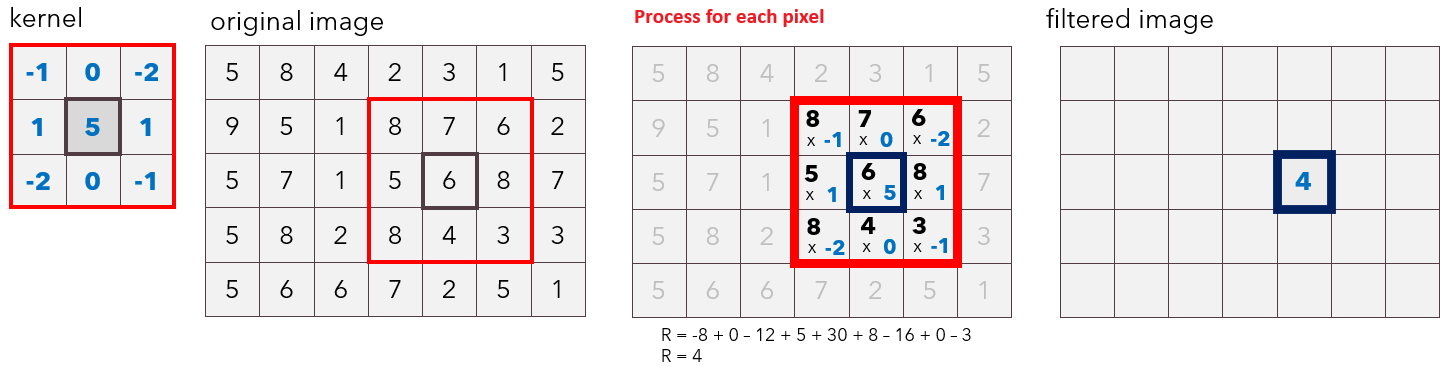
\includegraphics[width=\textwidth]{images/kernel.png}
\end{center}

Les éléments structurants jouent un rôle clé en traitement d'image, notamment dans les opérations de morphologie mathématique. Ces opérations sont principalement utilisées pour analyser et traiter des images binaires ou en niveaux de gris en modifiant leurs formes ou en extrayant des structures spécifiques.


\subsection{Filtre moyenneur gaussien}

\begin{mdframed}[style=sidebar,frametitle={}]
Notions : \href{https://iogs-lense-training.github.io/image-processing/contents/opencv_blur.html#blur-with-opencv
}{\textit{Blur with OpenCV}}
\end{mdframed}

\Manip Créer un nouveau projet sous PyCharm.

\Manip Impoter la bibliothèque \textbf{OpenCV2} (\textit{cv2}).

\Manip Ouvrir l'image \textsl{bricks2.jpg} du kit d'images fourni, en niveau de gris.

\Manip Appliquer un filtre gaussien (fonction \textsl{cv2.GaussianBlur()}) sur l'image précédente, de taille 5 x 5 pixels.

\Manip Afficher les deux images pour les comparer.

\Quest Comment peut-on montrer de manière objective les modifications apportées à l'image ? 

\Manip Mettre en oeuvre la méthode proposée.

\medskip

On se propose d'utiliser la fonction \textsl{compare\_blur\_fft()} fournie dans le fichier \textsl{images\_manipulation.py} pour comparer l'effet. 

Ce fichier est disponible sur le site du LEnsE dans la rubrique \textit{Année / Première Année / Interfaçage Numérique S6 / Bloc Images et OpenCV / Répertoire vers codes à tester}.

\Manip Tester cette fonction sur l'image précédente.

\Quest Etudier cette fonction. Quelles méthodes sont utilisées pour comparer les images ?

\Quest Quelle est la fonction réalisée par le filtre précédent ?

\medskip

On cherche à présent à voir l'impact du noyau sur l'image finale.

\Manip Tester la fonction précédente avec des noyaux de taille différente et comparer les résultats à la fois sur l'image obtenue mais également sur la transformée de Fourier.

\Quest Que pouvez-vous conclure sur l'impact de la taille du noyau ?


\subsection{Bruit sur une image}

On se propose d'étudier la fonction \textsl{generate\_gaussian\_noise\_image()} fournie dans le fichier \textsl{images\_manipulation.py}.

\Manip Tester l'exemple fourni dans le fichier \textsl{noise\_test1.py}.

\Quest Comment vérifier la distribution du bruit généré par cette fonction ?

\medskip

On se propose d'étudier la fonction \textsl{generate\_uniform\_noise\_image()} fournie dans le fichier \textsl{images\_manipulation.py}.

\Manip Tester l'exemple fourni dans le fichier \textsl{noise\_test2.py}.

\Quest La distribution du bruit généré par cette fonction est-elle uniforme ?

\Manip A l'aide de la fonction \textsl{generate\_gaussian\_noise\_image\_percent()}, générer un bruit gaussien de moyenne 30 et d'écart-type 20 sur 10\% de l'image \textsl{robot.jpg} ouverte précédemment en nuance de gris. Visualiser le résultat.

\medskip

\textit{Il peut-être nécessaire de normaliser les images bruitées afin que les \textbf{données entières} de chaque pixel soient comprises \textbf{entre 0 et 255}, afin que les images puissent être affichées correctement.} 

\Manip Tester la fonction \textsl{compare\_blur\_fft()} fournie dans le fichier \textsl{images\_manipulation.py} et comparer les résultats à la fois sur l'image obtenue mais également sur la transformée de Fourier.


%%%%%%%%%%%%%    Etape 5
\section{Appliquer un filtre passe-haut sur une image}

\begin{center} \textbf{\textit{Temps conseillé : 60 min}} \end{center}

Le \textbf{filtre moyenneur} précédent permet de conserver les \textbf{éléments à basse fréquence spatiale} dans l'image. C'est une méthode intéressante pour supprimer des bruits ponctuels (des éléments isolés et donc "rapides"). Il est également possible en choisissant un autre élément structurant de réaliser l'opération complémentaire qui supprime le fond continu et ne conserve que les transitions de fréquence spatiale élevée (bords d'un objet par exemple).

\medskip

Il est possible d'utiliser la fonction \textsl{cv2.filter2D()} pour appliquer un noyau particulier sur une image.

\subsection{Opérateur de Roberts}

L'opérateur de Roberts est l'un des premiers filtres de \textbf{détection de contours}. Il repose sur la convolution avec deux petits noyaux 2x2, conçus pour approximer les dérivées en diagonale de l'image.

Les noyaux de convolution sont les suivants :

$$K_x = \begin{bmatrix}
+1 & 0 \\
0 & -1
\end{bmatrix},
\quad
K_y =
\begin{bmatrix}
0 & +1 \\
-1 & 0
\end{bmatrix}.
$$

Il est alors possible de calculer l'amplitude du gradient par l'opération suivante: 

$$\text{Amplitude} = \sqrt{G_x^2 + G_y^2}$$ où $G_x$ est le résultat de la convolution de l'image par le noyau $K_x$ et $G_y$ le résultat de la convolution de l'image par le noyau $K_y$.

Une forte amplitude indique un contour ou un bord marqué. Une faible amplitude indique une région où l'intensité est relativement constante.

\medskip

\Manip Ecrire un script qui permet d'appliquer cette opération sur l'image \textsl{bricks2.jpg} du kit d'images fourni, en niveau de gris.

\Manip Visualiser l'image originale, le résultat du filtrage selon X et le résultat du filtrage selon Y.

\Quest Que pouvez-vous conclure sur l'effet de ce filtre ?

\subsection{Opérateur de Sobel}

L'opérateur de Sobel permet de réaliser une opération similaire à celui de Roberts, mais en étant moins sensible aux bruits dans l'image, puisqu'il se base sur un noyau plus large et ainsi lisse l'image dans la direction perpendiculaire au gradient mesuré.

Les noyaux de convolution sont les suivants :

$$G_x = \begin{bmatrix}
-1 & 0 & 1 \\
-2 & 0 & 2 \\
-1 & 0 & 1 
\end{bmatrix},
\quad
G_y =
\begin{bmatrix}
-1 & -2 & -1 \\
0 & 0 & 0 \\
1 & 2 & 1 
\end{bmatrix}.
$$

De la même façon que précédemment, on peut calculer l'amplitude du gradient par l'opération suivante : 

$$\text{Amplitude} = \sqrt{G_x^2 + G_y^2}$$ où $G_x$ est le résultat de la convolution de l'image par le noyau $K_x$ et $G_y$ le résultat de la convolution de l'image par le noyau $K_y$.

\medskip

\Manip Ecrire un script qui permet d'appliquer cette opération sur l'image \textsl{bricks2.jpg} du kit d'images fourni, en niveau de gris.

\Manip Visualiser l'image originale, le résultat du filtrage selon X et le résultat du filtrage selon Y.

\Quest Que pouvez-vous conclure sur l'effet de ce filtre ?

%%%%%%%%%%%%%    Etape 6
\section{Appliquer un filtre par l'intermédiaire de la transformée de Fourier}

\begin{center} \textbf{\textit{Temps conseillé : 30 min}} \end{center}

On s'intéresse ici à la \textbf{transformée de Fourier discrète en deux dimensions} permettant de représenter l'image dans le domaine fréquentiel, plutôt que dans le domaine spatial.

\Manip Ouvrir l'image \textsl{robot.jpg} du kit d'images fourni, en niveau de gris.

\Manip Calculer la transformée de Fourier discrète de cette image à l'aide de la fonction \textsl{fft2()} de la bibliothèque \textbf{Numpy / FFT}. Afficher l'image et sa transformée de Fourier. \textit{Pensez à utiliser la fonction fftshift...}

\medskip

On se propose d'utiliser la fonction \textsl{circular\_mask()} fournie dans le fichier \textsl{images\_manipulation.py} pour appliquer un masque sur la transformée de Fourier de l'image. 

Ce fichier est disponible sur le site du LEnsE dans la rubrique \textit{Année / Première Année / Interfaçage Numérique S6 / Bloc Images et OpenCV / Répertoire vers codes à tester}.

\Manip Appliquer un masque circulaire sur la transformée de Fourier de l'image, à l'aide de la fonction \textsl{circular\_mask()}. Afficher le résultat.

\Manip Calculer l'image résultante à l'aide de la fonction \textit{ifft2()} de la bibliothèque \textbf{Numpy / FFT}. Afficher l'image résultante et la comparer à l'image originale.

\medskip

\Manip Ecrire et tester une fonction permettant de réaliser un masquage rectangulaire sur une image, dont on pourra préciser la largeur et la longueur, ainsi que le barycentre du rectangle (point d'intersection des diagonales).

\Quest Que se passe-t-il lorsque vous appliquez un masque rectangulaire (dont la largeur et la longueur sont différentes) sur une image ? Qu'en est-il d'un masque circulaire ?


%%%%%%%%%%%%%%%%%%%%%%%%%%%%%%%%%%%%%%%%%%%%%%%%
%%% RESSOURCES COMPLEMENTAIRES	

\newpage
\begin{center}
	\begin{minipage}{2.5cm}
	\begin{center}
		
\includegraphics[width=5cm]{images/Logo-LEnsE.png}
	\end{center}
\end{minipage}\hfill
\begin{minipage}{10cm}
	\begin{center}
	\textbf{Institut d'Optique Graduate School }\\[0.1cm]
    \textbf{Interfaçage Numérique}


	\end{center}
\end{minipage}\hfill


\vspace{2cm}


{\Large \bfseries \textsc{Interfaçage Numérique}} \\[0.5cm]
{\large \bfseries Travaux Pratiques} \\[0.2cm]
Semestre 6

\vspace{1cm}

% Title
\rule{\linewidth}{0.4mm} \\[0.4cm]
{ \Large \bfseries\color{violet_iogs} Ressources \\[0.4cm] }
\rule{\linewidth}{0.4mm} \\[1cm]
{\large Bloc Caméra}

\end{center}

\vspace{3cm}



\textbf{\large Liste des ressources}
\begin{itemize}
	\item \hyperref[doc:image_proc]{Camera and sensor / Key concepts}
\end{itemize}

\vfill

\newpage
\strut % empty page


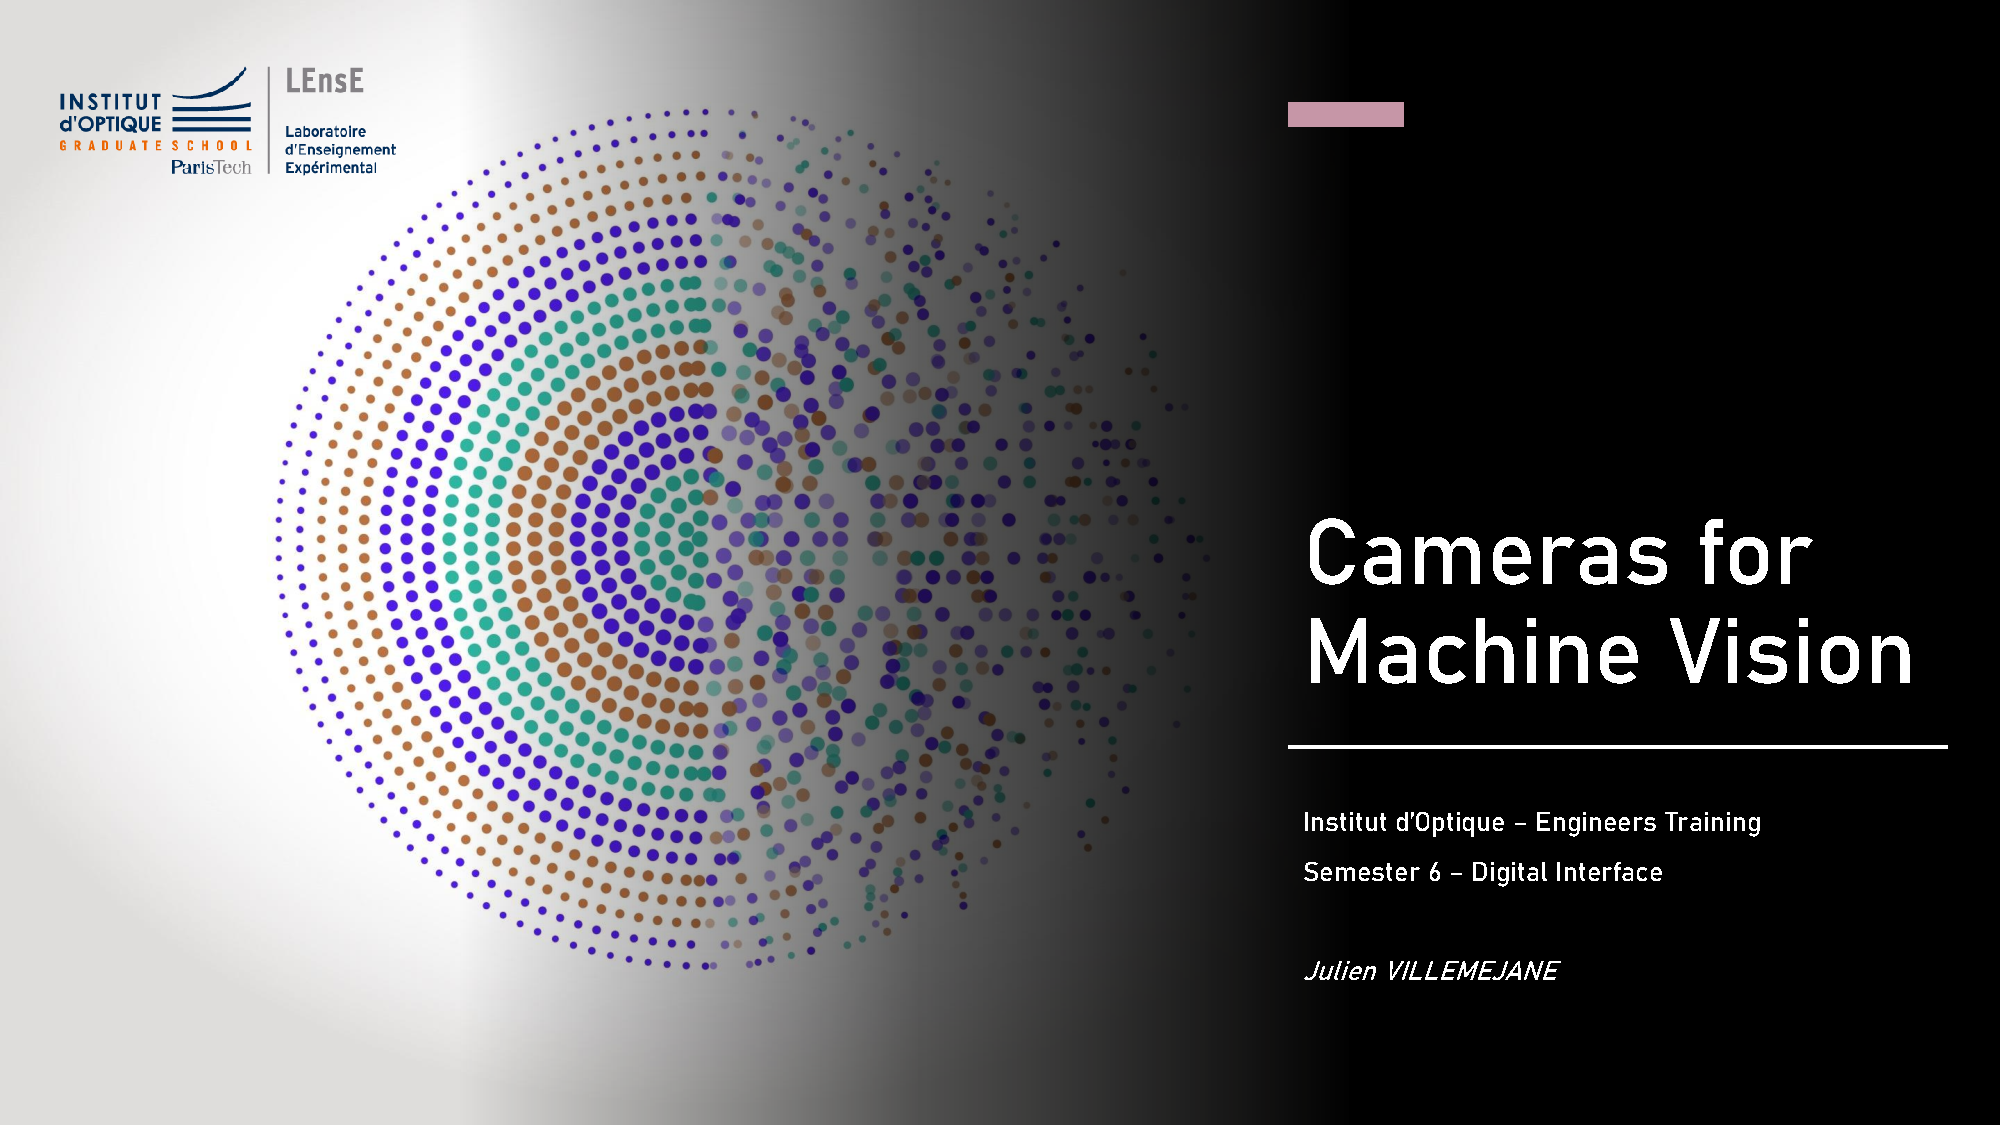
\includepdf[pages={1,3}, nup=1x2, pagecommand={\section{\texorpdfstring{\hspace{-1em}}{Camera and sensor}}}\label{doc:image_proc}]{../docs/Cameras.pdf}
\includepdf[pages={7,10-14,16,19,22,23,24,25,8}, nup=1x2]{../docs/Cameras.pdf}


\end{document}


